\chapter{\label{method}Theory}
In this chapter, the theoretical background will be detailed before we discuss the particulars of the experiment.
\section{Dynamics of Cyclical Systems}
The study of cyclical evolutions, where a system returns to its initial state at the end of the evolution, is a common topic in Physics. In quantum mechanics, the state vector of a system after a cyclical evolution is related to its initial state vector by a phase factor. This phase has a geometric component, which was first demonstrated by Pancharatnam in 1956 for cyclic evolution of the polarization state of light, and later by Berry in 1984 for adiabatic evolution of the Hamiltonian. The geometric phase for adiabatic evolution depends on the closed trajectory of the state ray in the Hilbert space and has been generalized to any cyclical evolution by Aharonov and Anandan. The geometric phase has been observed experimentally in various interference experiments, such as the Aharonov-Bohm effect, nuclear magnetic resonance, and laser optics. This concept has numerous applications, including the theory of insulators and quantum information.

This article focuses on a specific quantum mechanical system, a two-state atom interacting with a steadily oscillating electric field such as a laser, which exhibits Rabi oscillations and evolves cyclically. The article mathematically demonstrates that the motion of a system of two classical coupled oscillators is analogous to this quantum system. The periodic transfer of energy between the oscillators is similar to Rabi oscillations in the atom. This analogy is used to study the evolution of the oscillator as a trajectory on an equivalent Hilbert space and to obtain the associated geometric phase. The article also describes a simple experiment suitable for undergraduate students to demonstrate and measure the geometric phase, with the measured value found to be in good agreement with the expected phase. This analogy has been previously demonstrated in electrical RLC circuits to show phenomena such as electromagnetically induced transparency (EIT), double EIT, and Fano interference. The article concludes by noting that the use of analogies between classical and quantum mechanical systems is a topic of ongoing research and discussion.

\section{Theoretical Framework}
\begin{figure}[H]
	\centering
	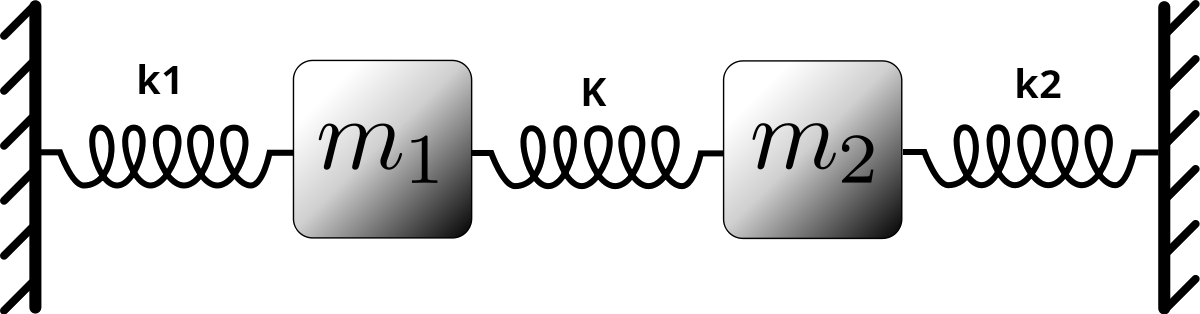
\includegraphics[scale=0.3]{coupled1.png}
	\caption{The amplitude versus current data obtained for Fe rod on the magnetic bench}
	\label{fig:mb-fe-0}
\end{figure}
$$ \begin{array}{l}m_{1} \ddot{x}_{1}=-k_{1} x_{1}+k\left(x_{2}-x_{1}\right), \\ m_{2} \ddot{x}_{2}=k\left(x_{1}-x_{2}\right)-k_{2} x_{2} .\end{array}$$
$$-\frac{\mathrm{d}^{2}}{\mathrm{~d} t^{2}} \boldsymbol{\xi}=\mathbf{A} \boldsymbol{\xi}$$
$$ \boldsymbol{\xi}=\left(\begin{array}{l}\tilde{x}_{1} \\\tilde{x}_{2}\end{array}\right) \quad \text { and } \quad \mathbf{A}=\left(\begin{array}{cc}\omega_{1}^{2} & -\Omega_{1}^{2} \\-\Omega_{2}^{2} & \omega_{2}^{2}\end{array}\right),$$
$$\omega_{ \pm}^{2}=\frac{1}{2}\left(\omega_{1}^{2}+\omega_{2}^{2} \pm\left[4 \Omega_{1}^{2} \Omega_{2}^{2}+\left(\omega_{1}^{2}-\omega_{2}^{2}\right)^{2}\right]^{1 / 2}\right) .$$
$$
\boldsymbol{\xi}(t)=F_{+} \boldsymbol{\xi}_{+} \exp \left(-\mathrm{i} \omega_{+} t-\mathrm{i} \phi_{+}\right)+F_{-} \boldsymbol{\xi}_{-} \exp \left(-\mathrm{i} \omega_{-} t-\mathrm{i} \phi_{-}\right),$$
The quantum two level system\\
\begin{figure}[H]
	\centering
	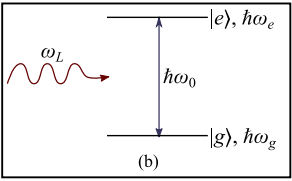
\includegraphics[scale=1]{two level.png}
	\caption{The amplitude versus current data obtained for Fe rod on the magnetic bench}
	\label{fig:mb-fe-0}
\end{figure}
The system illustrated in figure 1(b)\footnote{ Sharba Bhattacharjee et al 2018 Eur. J. Phys. 39 035404} is that of an atom with a ground state\ \( |g\rangle \) of energy \( \hbar \omega_{g} \) and an excited state \( |e\rangle \) of energy \( \hbar \omega_{e} \), with resonant frequency \( \omega_{e}-\omega_{g}=\omega_{0} \). It interacts with an oscillating electric field \( \mathcal{E}(t)=\operatorname{Re}\left(\mathcal{E}_{0} \mathrm{e}^{\mathrm{i} \omega_{L} t}\right) \) such as a single-mode laser. We define the dipole moment \( \mu=e\langle g|\mathbf{r} \cdot \hat{\mathcal{E}}| e\rangle \), where \( e \) is the electronic charge and \( \hat{\mathcal{E}} \) is the unit vector in the direction of the electric field. Then the Hamiltonian matrix of the system in the \( \{|g\rangle,|e\rangle\} \) basis is [12]\[\mathbf{H}=\left(\begin{array}{cc}\hbar \omega_{g} & -\mu \mathcal{E}(t) \\-\mu^{*} \mathcal{E}(t) & \hbar \omega_{e}\end{array}\right)\]If we transform the state vector using the unitary operator \( U=|g\rangle\left\langle g\left|+\mathrm{e}^{-\mathrm{i} \omega_{L} t}\right| e\right\rangle\langle e| \), then the Hamiltonian matrix elements in the new basis \( \left\{|\tilde{g}\rangle=U^{\dagger}|g\rangle=|g\rangle,|\tilde{e}\rangle=U^{\dagger}|e\rangle=\mathrm{e}^{\mathrm{i} \omega L t}|e\rangle\right\} \) become time independent under the rotating wave approximation,\[\tilde{\mathbf{H}}=\hbar\left(\begin{array}{cc}\omega_{g} & -\Omega / 2 \\-\Omega / 2 & \omega_{g}+\Delta\end{array}\right)\]where we have defined \( \Delta=\omega_{0}-\omega_{L} \) (called the detuning) and \( \Omega=\mu \mathcal{E}_{0} / \hbar \) (called the Rabi frequency). \( \Omega \) is in general a complex quantity depending on the phase of the laser; here we choose the phase to be zero so that \( \Omega \) is real. Physically, this may be interpreted as moving the laser source towards or away from the atom to ensure that \( \mu \mathcal{E}_{0} \) is real. Then the state \( |\tilde{\psi}(t)\rangle \) of the system at a time \( t \), with the initial condition \( |\tilde{\psi}(0)\rangle=|\tilde{g}\rangle \), is given in the \( \{|\tilde{g}\rangle,|\tilde{e}\rangle\} \) basis as \( [12] \)\[|\tilde{\psi}(t)\rangle=c_{1}(t)|\tilde{g}\rangle+c_{2}(t)|\tilde{e}\rangle \equiv\left(\begin{array}{l}c_{1}(t) \\c_{2}(t)\end{array}\right),\]where\[\begin{aligned}c_{1}= & \frac{1}{2}\left[\left(\sqrt{\Delta^{2}+\Omega^{2}}-\Delta\right) \exp \left(-\mathrm{i}\left(\Delta+\sqrt{\Delta^{2}+\Omega^{2}}\right) t / 2-\mathrm{i} \omega_{g} t\right)\right. \\& \left.+\left(\sqrt{\Delta^{2}+\Omega^{2}}+\Delta\right) \exp \left(-\mathrm{i}\left(\Delta-\sqrt{\Delta^{2}+\Omega^{2}}\right) t / 2-\mathrm{i} \omega_{g} t\right)\right]\left(\Delta^{2}+\Omega^{2}\right)^{-1 / 2} \\c_{2}= & \frac{1}{2}\left[\Omega \exp \left(-\mathrm{i}\left(\Delta-\sqrt{\Delta^{2}+\Omega^{2}}\right) t / 2-\mathrm{i} \omega_{g} t\right)\right. \\& \left.-\Omega \exp \left(-\mathrm{i}\left(\Delta+\sqrt{\Delta^{2}+\Omega^{2}}\right) t / 2-\mathrm{i} \omega_{g} t\right)\right]\left(\Delta^{2}+\Omega^{2}\right)^{-1 / 2}\end{aligned}\]The coefficients \( c_{1}(t) \) and \( c_{2}(t) \) are the probability amplitudes, so that at any given time \( t \), \( \left|c_{1}(t)\right|^{2} \) and \( \left|c_{2}(t)\right|^{2} \) are the probabilities of the system collapsing to the states \( |\tilde{g}\rangle \) and \( |\tilde{e}\rangle \) respectively if its energy is measured.


% Please add the following required packages to your document preamble:
% \usepackage{booktabs}
\begin{table}[]
	\centering
	\caption{}
	\label{tab:systems}
	\resizebox{\textwidth}{!}{%
	\begin{tabular}{@{}ll@{}}
		\toprule
		\textbf{Coupled oscillator} & \textbf{Two-level system} \\ \midrule
		Squares of amplitudes \( \left|\tilde{x}_{1}\right|^{2},\left|\tilde{x}_{2}\right|^{2} \) & Probabilities \( \left|c_{1}\right|^{2},\left|c_{2}\right|^{2} \) \\
		First natural frequency \( \omega_{1} \) & \( \left(\omega_{g}^{2}+\Omega^{2} / 4\right)^{1 / 2} \) \\
		Second natural frequency \( \omega_{2} \) & {\( \left[\left(\omega_{g}+\Delta\right)^{2}+\Omega^{2} / 4\right]^{1 / 2} \)} \\
		Coupling \( \Omega_{1}=\Omega_{2} \) & \( \left[\Omega\left(2 \omega_{g}+\Delta\right) / 2\right]^{1 / 2} \) \\ \bottomrule
	\end{tabular}%
}
\end{table}


Scale 1 is $ k_1 $ 
scale 2 is $ k_2 $
rubberband is $ K $
the extra rubberband we use changes $ k_2 $ but it also changes how quickly the system is damped


\section{Modelling the coupled oscillator}

The following equation was used to model the coupled oscillator:

\begin{equation}
	f (t) = A \cos [ \omega_{+} (t - d) + \phi ] + B \cos [ \omega_{-} (t-d) \phi ] +C
\end{equation}

The fitted values of $ A $, $ B $, $ \omega_{+} $ and $ \omega_{-} $ are used to calculate the parameters $ \omega_g $, $ \Delta $ and $ \Omega $ of the Rabi model as

\begin{equation}
	\begin{split}
		\Delta &= (\omega_{+} - \omega_{-}) \dfrac{B-A}{B+A}, \\
		\Omega &= (\omega_{+} - \omega_{-}) \Bigg[ 1 - \Bigg(  \dfrac{B-A}{B+A} \Bigg)^2  \Bigg]^{1/2}, \\
		\omega_g &= \dfrac{\omega_{+} + \omega_{-} - \Delta}{2}
	\end{split}
\end{equation}

Further we calculte the geometric phase as

\begin{equation}
	\phi_G = \pi \Bigg( 1 - \dfrac{\Delta}{\sqrt{\Delta^2 + \Omega^2 }} \Bigg)
\end{equation}

\section{The action of the coupling agent}
When you stretch a rubber band there is considerable deformation to the polymer molecules in the rubber. As a result some of the work you do on the rubber band goes into exciting molecular vibrations i.e. heat. Some of the work you do is stored as elastic energy and some is dissipated as heat.

As the band is allowed to relax the elastic energy stored within it does work on you. However, as before some of this energy goes into molecular vibrations and some into heat.

In both cases the work is the integral of force with distance, i.e. the area under a force-distance graph, however, this graph will show some hysteresis due to the energy that is dissipated as heat\footnote{Source:John Rennie, Net work done for rubber bands, https://physics.stackexchange.com/q/149122}:
\begin{figure}[H]
	\centering
	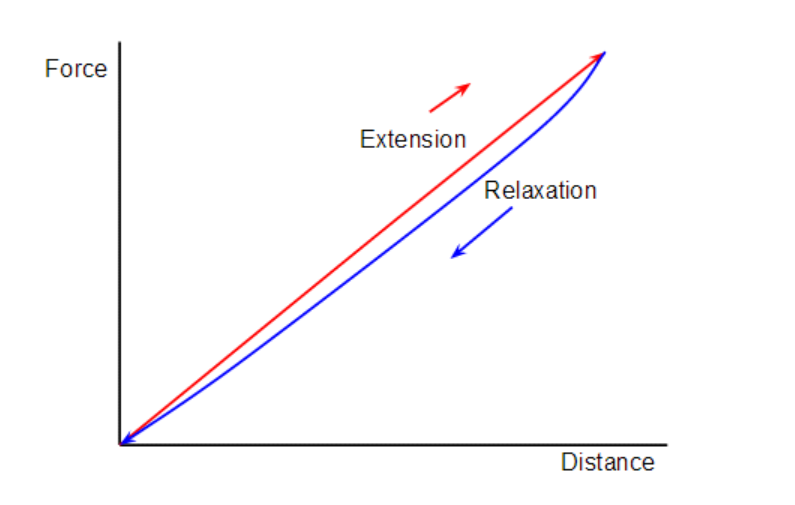
\includegraphics[scale=0.5]{Rubberband hysteresis.png}
	\caption{The amplitude versus current data obtained for Fe rod on the magnetic bench}
	\label{fig:mb-fe-0}
\end{figure}
Because of the hysteresis you don't get as much work out as you put in and the net work is not zero.

In the case of permanent deformation the physics is basically similar, except that the difference between the extension and relaxation force-distance curves is greater so more work is lost as heat.

\section{The Correlation Matrix}

Suppose we have an equation with multiple parameters and we are trying to fit some dataset to this equation. In probability theory and statistics, it is essential to realise that there might be some correspondence between two of those parameters, even if they are independent in the physical sense. We define this property as \textit{covariance}. It is the join variablity of two random variables. The greater two parameters correspond or correlate with each other, the higher will be the covariance.

We can construct a matrix that contains all the information about the covariance or correlation between all the pairs of parameters of an equation. A square matrix which can represent all the covariance values of all the pairs of aparameters of the equation is called the covariance or correlation matrix. So, if the entries of the column vector 

\begin{equation}
	\mathbf{X} = (X_1, X_2, \ldots, X_n,)^{T}
\end{equation}
are random variables, each with finite variance and expected value, then the covariance matrix $ K_{XX} $ is the matrix whose $ (i, j) $ entry is the covariance
\begin{equation}
	K_{X_i X_j} = \text{cov} [X_i, X_j]	= E [(X_i - E[X_i])(X_j - E[X_j])]
\end{equation}
where $ E $ is an operator which denotes the expected value (mean) of its argument.

In our analysis, we used Python's \texttt{SciPy} library's \texttt{curve\_fit} function. This function returns a tuple containing the two arrays. The first array contains the optimal parameters of the fittef function. The second array is a 2-D array, which represents the covariance matrix. 

Note that the diagonal values of the covariance matrix give us the standard deviation in the parameters and the off-diagonal elements represents the covariance between $ (i, j) $ pairs. Therefore, if all the off-diagonal values are sufficently small, we can conclude it is a good quality fit.
%\baselineskip 24pt



    



